\documentclass[12pt]{article}
\pagestyle{empty}
\usepackage{amsmath, amssymb, amsthm}
\usepackage{latexsym, epsfig, ulem, cancel, multicol, hyperref}
\usepackage{graphicx, tikz, subfigure,pgfplots}
\usepackage[margin=1in]{geometry}
\setlength{\parindent}{0pt}
\usepackage{multirow}
\usepackage{mathtools}
\usepackage{verbatim}
\usepackage{tikz}
\usepackage{pgfplots}
\setlength{\parskip}{1ex}

\newcommand{\T}[0]{\top}
\newcommand{\F}[0]{\bot}
\newcommand{\liminfty}[1]{\lim_{#1 \to \infty}}
\newcommand{\limzero}[1]{\lim_{#1 \to 0}}
\newcommand{\limto}[1]{\lim_{#1}}
\newcommand{\Z}{\mathbb{Z}}
\newcommand{\R}{\mathbb{R}}
\newcommand{\C}{\mathbb{C}}
\newcommand{\Q}{\mathbb{Q}}
\newcommand{\odd}[0]{\mathbb{Z} - 2\mathbb{Z}}
\newcommand{\lineint}[1]{\int_{#1}}
\newcommand{\pypx}[2]{\frac{\partial #1}{\partial #2}}
\newcommand{\divg}{\nabla \cdot}
\newcommand{\curl}{\nabla \times}
\newcommand{\dydx}[2]{\frac{\text{d} #1}{\text{d} #2}}
\newcommand{\sqbkt}[1]{\left[ #1 \right]}
\newcommand{\paren}[1]{\left( #1 \right)}
\newcommand{\tribkt}[1]{\left< #1 \right>}
\newcommand{\abso}[1]{\left|#1 \right|}
\newcommand{\zero}{\{0\}}
\newcommand{\then}{\rightarrow}
\newcommand{\nonneg}{\Z^+ \cup \{0\}}
\DeclarePairedDelimiter\ceil{\lceil}{\rceil}
\DeclarePairedDelimiter\floor{\lfloor}{\rfloor}
\newcommand{\union}[2]{\bigcup_{#1}^{#2}}
\newcommand{\inter}[2]{\bigcap_{#1}^{#2}}
\newcommand{\openclose}[1]{\left( #1 \right]}
\newcommand{\closeopen}[1]{\left[ #1 \right)}
\newcommand{\compo}[2]{#1 e^{i #2}}
\newcommand{\laplase}{\bigtriangleup}
\newcommand{\bra}[1]{\left< #1 \right|}
\newcommand{\ket}[1]{\left| #1 \right>}
\newcommand{\braket}[2]{\left< #1 \mid #2 \right>}
\newcommand{\ketbra}[2]{\left| #1 \right> \left< #2 \right|}
\newcommand{\ketpsit}{\ket{\psi(t)}}
\newcommand{\ketphit}{\ket{\phi(t)}}
\newcommand{\ham}{\mathbf{H}}
\newcommand{\unx}{\hat{\mathbf{x}}}
\newcommand{\uny}{\hat{\mathbf{y}}}
\newcommand{\uns}{\hat{\mathbf{s}}}
\newcommand{\unr}{\hat{\mathbf{r}}}
\newcommand{\untheta}{\hat{\boldsymbol\theta}}
\newcommand{\unphi}{\hat{\boldsymbol\phi}}

\newcommand{\wsnumber}{1}
\newcommand{\wstopic}{Vectors}
\pgfplotsset{
    every linear axis/.append style={
       axis x line=center,
       axis y line=center,
       xlabel={$x$},
       ylabel={$y$}
    },
    every axis plot/.append style={thick,mark=none}
}
\tikzset{
    point/.style={circle,draw,fill,minimum width=0.3ex,inner sep=0pt,outer sep=0pt},
    every label/.append style={black}
}


\usepackage[margin=1in]{geometry}
\usepackage{amsmath, amssymb, amsthm, graphicx, hyperref}
\usepackage{enumerate}
\usepackage{fancyhdr}
\usepackage{multirow, multicol}
\usepackage{tikz}
\pagestyle{fancy}
\fancyhead[RO]{Dennis Li}
\fancyhead[LO]{Analytical Mechanics }
\usepackage{comment}
\newif\ifshow
\showfalse

\ifshow
  \newenvironment{solution}{\textbf{Solution.}}{}
\else
  \excludecomment{solution}
\fi

\renewcommand{\thefootnote}{\fnsymbol{footnote}}
\usepackage{comment}


\newtheorem*{remark}{Remark}


\begin{document}
\begin{center}
\ifshow
  \textbf{\Large Problem Set 03 Solution}\\
\else
  \textbf{\Large Problem Set 03}\\
\fi
Instructor \\ Prof. Gabe\\
\end{center}

\hrule

\vspace{0.2cm}


\section{1 Nostalgia}
Here are a couple of tougher problems that you could/should have seen in your intro-level course but probably did not:

\begin{itemize}
    \item T1 4.8: Consider a small frictionless puck perched at the top of a fixed sphere of radius $R$. If the puck is given a tiny nudge so that it begins to slide down, through what vertical height will it descend before it leaves the surface of the sphere? \textit{[Hint: Use conservation of energy to find the puck's speed as a function of its height, then use Newton's second law to find the normal force of the sphere on the puck. At what value of this normal force does the puck leave the sphere?]}

    The ball will leave the surface when the centripetal force is equivalent to the normal force of the surface. We can use the energy conservation to find the puck's height as a function of time. If we set the height of the puck at the top of the sphere to be $R$, and let the ground be $y=r$, we can express the potential energy of the puck at the top of the sphere as
    \[
    U = mgR
    \]
    We know that the total energy at the top of the sphere is given as
    \[
    E = mgR
    \]
    And the energy is conserved throughout the fall, therefore
    \[
    E = U+K
    \]
    This means
    \[
    mgR = mgh + \frac{1}{2}m\mathbf{v}^2
    \]
    From geometry we know that we can express the height of the puck as
    \[
    h = R\cos\theta
    \]
    Where $\theta$ is the angle of deviation from the $\uny$ axis. Now, we can work out the equation a little more
    \[
    2gR = 2gR\cos\theta + \mathbf{v}^2
    \]
    This means that
    \[
    \mathbf{v}^2 = 2gR\paren{1-\cos\theta}
    \]
    Now, we want to express the relationship between the gravitational force and the normal force. From the angle we defined, we have
    \[
    F_N = F_g\cos\theta = mg\cos\theta
    \]
    We also know that the centripetal force on a circular motion is
    \[
    F_c = \frac{m\mathbf{v}^2}{R}
    \]
    The puck leaves when the normal force and the centrepetal force is the same
    \[
    \frac{m\mathbf{v}^2}{R} = mg\cos\theta
    \]
    We can substitute our previous result for $\mathbf{v}^2$, this gives us
    \[
    \frac{2gR\paren{1-\cos\theta}}{R} = mg\cos\theta
    \]
    After some simplification, we have
    \[
    2-2\cos\theta = \cos\theta
    \]
    This means that
    \[
    \cos\theta = \frac{2}{3}
    \]
    And if we substitute this value back to the expression for height, we have
    \[
    h_{c} = \frac{2}{3}R
    \]
    \newpage
    \item MT5 2-25: 
A block of mass $m = 1.62$ kg slides down a frictionless incline (Figure 1). The block is released from a height $h = 3.91$ m above the bottom of the loop.

\begin{enumerate}
    \item[(a)] What is the force of the inclined track on the block at the bottom (point A)?
    
    Since all the potential energy is converted into kinetic at the bottom of the incline, or point A, I would like to analyze a situation that is analogous to this particular one. Suppose we have a quarter circular incline of radius $h$, and the puck all off from the height $h$ along the incline. The total energy is
    \[
    E = mgh
    \]
    By conservation of energy, we know that
    \[
    E = K + U = \frac{1}{2}m\mathbf{v}^2 + mgh(1-\cos\theta) = mgh
    \]
    Where $\theta$ is the angle of the centripetal force makes with the vertical axis $y$. 

    With some manipulation, we have
    \[
    \mathbf{v}^2   = 2gh\cos\theta
    \]
    Throw this into the equation for centripetal force in a circular motion, we have
    \[
    F_c = \frac{m\mathbf{v}^2 }{h} = 2mg\cos\theta
    \]

    Since at the bottom of the decline, all the energy is converted into kinetic, we have that
    \[
    mgh = \frac{1}{2}m\mathbf{v}^2
    \]
    This gives us
    \[
    \mathbf{v}^2 = 2gh
    \]
    At this point, the centripetal force is given by
    \[
    F_c = \frac{m\mathbf{v}^2}{h} = \frac{2mgh}{h} = 2mg
    \]
    And the net force is given by
    \[
    F_{net} = F_c + F_{g,c} 
    \]
    where $F_{g,c}$ is the reaction from the incline of the block's gravitational force. Therefore, the net force is
    \[
    F_{net} = 2mg + mg = 3mg
    \]
    We see that this expression of the net force on the bottom of the incline does not depend on the radius of the circular motion, therefore I claim that this is an analogous case in our scenario in Figure $1$. Therefore, the force of the incline on the block from the incline at pont $A$ is
    \[
    F_{i,b} = 3mg
    \]

    
    \item[(b)] What is the force of the track on the block at point B?

    With the previously established knowledge that the force does not depend on the radius of the cirular path, but the angle, we can simply use the result we obtained from previous section
    \[
    F_{net,block} = F_{c} + F_{N} = 2mg\cos\theta + F_N
    \]
    Now we only need to find the normal force. But we know that the normal force is only related to the gravitational force and the angle, we have the following relationship
    \[
    F_N = F_g\cos\theta = mg\cos\theta
    \]
    Therefore we have the general expression for the net force on the circular path.
    \[
    F_{net,block} = 3mg\cos\theta
    \]
    We see that this does not depend on the radius $R$. And we can simply throw in $\theta = 45^\circ$ to obtain the final result.
    \[
    F_{net,block} = \frac{3mg}{\sqrt{2}}
    \]
    \item[(c)] At what speed does the block leave the track?

    The block will have the same speed entering
    
    \item[(d)] How far away from point A does the block land on level ground?
    \item[(e)] Sketch the potential energy $U(x)$ of the block. Indicate the total energy on the sketch.
\end{enumerate}

\begin{figure}[!h]
    \centering
    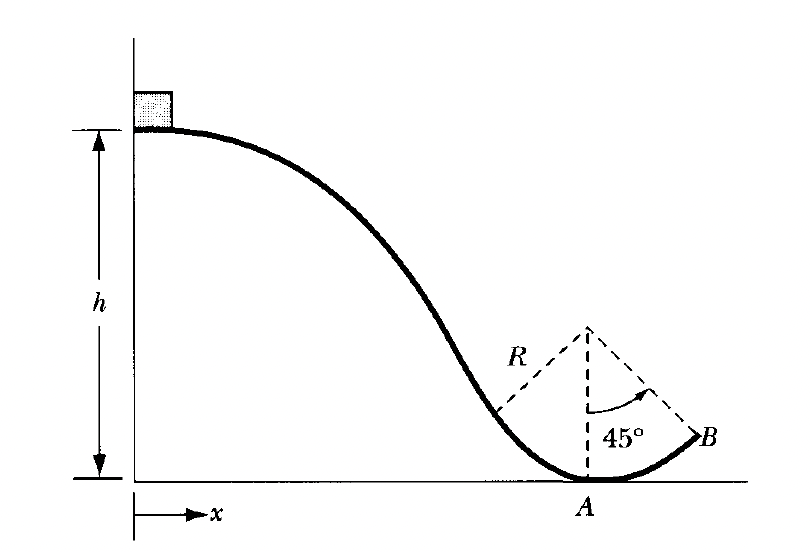
\includegraphics[width=0.5\linewidth]{Pictures//PS02/MT5-2-25.png}
    \caption{Enter Caption}
    \label{fig:MT2-25}
\end{figure}

\end{itemize}

\section*{2. 1 graph, 1 hill}

Consider two worlds:

\subsection*{World A:}
World A is 2D. Uniform surface gravity (of magnitude \(g\)) points in the \(-\hat{y}\) direction as usual in this world. There is a frictionless hill whose profile from the side has the shape \(y = y(x)\). A particle is confined to move along the surface of the hill (by a track or something). A particle of mass \(m\) is placed at \((x = 0, y = y(0))\) on the hill and released from rest. It moves.

\subsection*{World B:}
World B is 1D (x-axis only) and frictionless. A particle of mass \(m\) in this world is subject to a 1D force that has an associated potential energy function \(U(x) = mgy(x)\), where \(y(x)\) is the same function that describes the 2D hill in World A. That particle is placed at \(x = 0\) and released from rest. It moves.

For each of the following quantities, state whether they are the same or different in Worlds A \& B. Justify your answers. If they’re different, state whether the quantity is greater/equal/lesser in World A than World B or whether it depends on other information we don’t have (and identify what that information would be, if you can).

\begin{enumerate}
    \item The net force on the particle at \(x = 0\).

        The net force on the particle at $x=0$ should be the same across the two world. We can try to justify this algebraically. First, we look at world. The net force would be given by the following relationship
        \[
        \mathbf{F}_{net} = \mathbf{F}_g + \mathbf{F}_N =
        \]
        Let the angle of the slope be $\theta$, then, we also know that the net force has the following magnitude
        \[
        \mathbf{F}_{net} = \mathbf{F}_g\sin\theta = -mg\sin\theta
        \]
        If the angle $\theta$ is small, we can have the following approximation
        \[
        \tan\theta \approx \sin\theta \approx \theta \approx \dydx{y}{x}
        \]
        We have arrived at
        \[
        \mathbf{F}_{net} = -mg\dydx{y}{x}
        \]
        The sum of normal force and the gravitational force should provide the net force, since the particle is not under any other forces. We know that the normal force is always orthogonal to the direction of motion since it is not a conserved force, and will not contribute to the change in energy. 

        In world B, the force experienced by the particle is given by the following
        \[
        \mathbf{F}_{net} = -\dydx{U}{x} = -\paren{\dydx{mgy}{x}} = -mg\dydx{y}{x}
        \]
        We see that the forces in two worlds is equivalent, but only for some gentle angle $\theta$. If the approximation is no longer viable due to larger $\theta$, the net force should not be the same. 

        But this has shown that they are fundamentally different forces in world A and B. 
        
    \item The \(x\)-component of the net force on the particle at \(x = 0\).

        I would say that they are essentially different force, since $x$ component in world A and world B describes very different forces. The $x$ component of the net force in world B is the net force, while in world A it is not the case. 
    
    \item The \(x\)-component of the net force on the particle at arbitrary \(x\) along its ensuing motion.
        I would say regardless of where the particle is located, the $x$ component of the net force measured is fundamentally different. Since the normal force $F_N$ is not conservative and does no work, it does not influence the energy of the system by any means, therefore it is not present in world B. Thus, regardless of where the particle is during its motion, they will be different due to the way forces is considered in two world.
    
    \item The speed of the particle at \(x = 0\).

        The speed at $x=0$ is $v_0 = 0$ in both world since the y are both released from rest. 

    \item The \(x\)-component of the particle’s velocity at \(x = 0\).

        The $x$ component of velocity in world B would be its total speed since we are looking at one dimensional motion. And it can be found by conservation of energy
        \[
        U(0) = mgy(0) = mgy(x) + \frac{1}{2}mv^2(x)
        \]
        And we find that
        \[
        v(x) = \sqrt{2\paren{gy(0) - gy(x)}}
        \]
        And the $x$ component in world A is defined in a completely different way and the $x$ component of velocity is just different. 
    
    \item The speed of the particle at arbitrary \(x\) along its ensuing motion.

        With conservation of energy, we can conclude that the total speed of the particle would be the same across tow frames, since we can use the same derivation above for both world.

    \item The \(x\)-component of the particle’s velocity at arbitrary \(x\) along its ensuing motion.

        The velocity is different just as we discussed previously. 
    
    \item The \(x\)-coordinate of the next place the particle stops during its ensuing motion.

        This should be the same across both world. Where ever the particle stops.
        
    \item The \(x\)-coordinates of all places where the particle stops during its ensuing motion.

        This should be the same across both world. Where ever the particle stops.
        
    \item The set of all \(x\)-coordinates visited by the particle during its ensuing motion.
    
        This should be the same across both world. Where ever the particle stops. They will cover the same distance in both world. 
        
\end{enumerate}

\section{Practice with 1D potentials}

\subsection{1 potential, many parts}
Consider a particle restricted to the region \( x > 0 \) moving in a 1D potential

\[
U(x) = U_0 \left( \frac{x}{a} - \frac{a}{x} \right) .
\]

\begin{enumerate}
    \item What are the dimensions of \(a\) and \(U_0\)?
        We know that $U$ has unit $J$ or joules. In S.I. units, we have
        \[
        1\,\text{J} = 1 \,\text{kg}\cdot\frac{\text{m}^2}{\text{s}^2}
        \]
        Logically, the initial energy $U_0$ has the dimension of $J$. Therefore $\frac{x}{\alpha}$ should be dimensionless. This means it should have the dimension of $\text{m}^{-1}$.
        
    \item Sketch the potential \(U(x)\).

    \begin{figure}[!h]
        \centering
        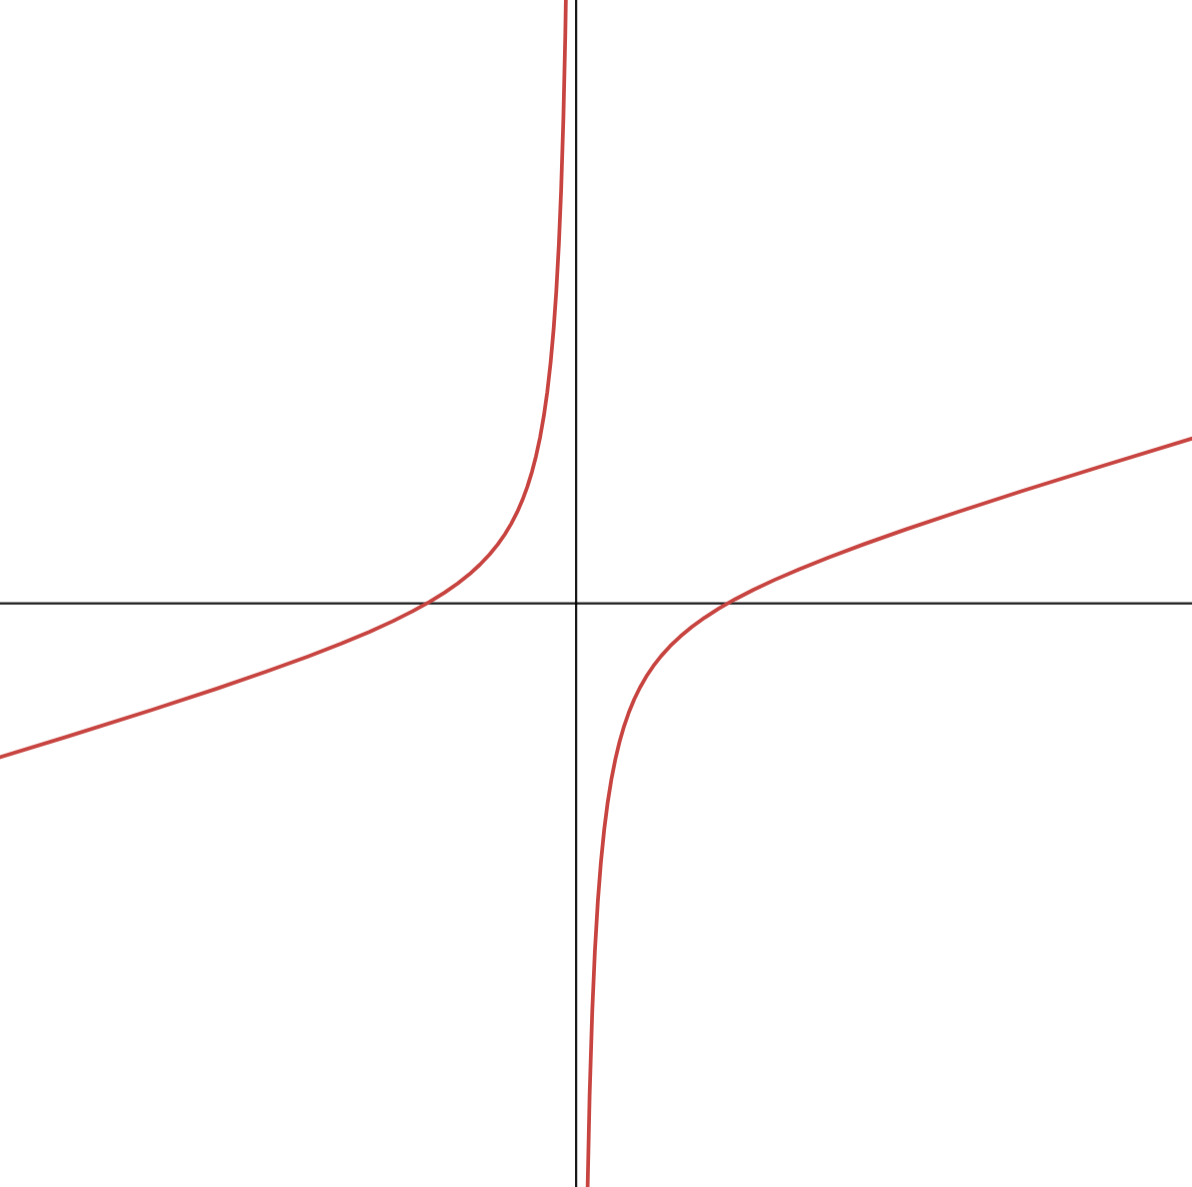
\includegraphics[width=0.5\linewidth]{Pictures//PS02/PS02-2-1.png}
        \caption{A Sketch of the Potential}
        \label{fig:ps02-2-1}
    \end{figure}
    
    \item Determine all equilibrium points and assess their stability.

    The Equilibrium can be found by taking the first derivative of the potential, or where the force is zero. 
    \[
    F(x) = -\dydx{}{x}\sqbkt{U_0 \left( \frac{x}{a} - \frac{a}{x} \right)}
    \]
    This evaluates to
    \[
    F(x) = -U_0\paren{\frac{1}{a} + \frac{a}{x^2}}
    \]
    We see that this equation has real root for $F(x) = 0$, therefore it does not seem to have an equilibrium.

    
    
\end{enumerate}

\subsection{1 force, many parts}
Consider a particle in 1D moving under the influence of a force

\[
F(x) = -kx + k \frac{x^3}{\alpha} ,
\]

where \(k\) and \(\alpha\) are constants and \(k > 0\) (this is a 1D force, so signs indicate direction, i.e. \(F < 0\) corresponds to a push in the \(-x\) direction).

\begin{enumerate}
    \item What are the dimensions of \(k\) and \(\alpha\)?
    \item Determine the potential \(U(x)\) and roughly sketch it.
    \item Qualitatively discuss the types of motion for different values of the total energy.
    \item What motions are allowed when the energy is exactly \(E = \frac{k \alpha}{4}\)?
\end{enumerate}






\end{document}